\documentclass[12pt]{article}

\usepackage[margin=1in]{geometry}
\usepackage{setspace}
\usepackage{booktabs}
\usepackage{graphicx}
\usepackage{parskip}
\usepackage[hidelinks]{hyperref}
\usepackage{titlesec}
\usepackage{enumitem}
\usepackage{float}
\usepackage{tikz}
\usepackage[
    style=apa,
    backend=biber,
    natbib=true,
    maxcitenames=2,
    mincitenames=1
]{biblatex}

\addbibresource{NLP_immigrantmentalhealth.bib}
\usetikzlibrary{shapes.geometric,arrows.meta,positioning,fit}

\titleformat{\section}{\normalfont\large\bfseries}{\thesection.}{0.6em}{}
\titleformat{\subsection}{\normalfont\normalsize\bfseries}{\thesubsection}{0.6em}{}

\title{\textbf{Contingent Lives: Visa Status and Distress Among Temporary Migrants}}
\date{PAA 2027 Submission}

\begin{document}

\maketitle

\section*{Abstract}
Temporary visa holders constitute a large but understudied population of documented migrants whose legal status remains
conditional on education, employment, or family relationships. Drawing on the concept of liminal legality, this study asks
how such conditional legal status may shape psychological distress beyond the deportation threat emphasized in research
on undocumented migration. Specifically, we ask how psychological distress is expressed among temporary visa holders and
what conditions participants themselves connect to distress, and whether these patterns differ by visa category, gender,
and household position. Drawing on 180 semi-structured interviews with F-1, H-1B, H-4, and F-2 visa holders in the United States, we will use
structured coding and latent class analysis to identify patterns of distress and the conditions participants associate
with them. We will then compare these patterns across visa categories, gender, and household position. By examining both the expression of distress and participants' own attributions of its sources, this study will provide
empirical evidence on how conditional legal status is experienced among documented temporary migrants.

\vspace{0.5em}
\noindent\textit{[143 words]}

\vspace{1.5em}
\hrule
\vspace{1.5em}

\section*{Extended Abstract}

\section{Motivation and Framing}
How does legal status shape psychological distress when migrants are formally authorized to remain but lack durable control
over their future? Research on immigration and mental health has largely centered on refugee and asylum seekers, emphasizing
deportability as a central mechanism of distress \citep{hamiltonLegalStatusDeportation2023, newnhamMentalHealthEffects2019}.
Yet research on refugees and asylum seekers suggests that liminal legality—legally recognized but conditional and potentially
unstable status—may generate distress through prolonged
uncertainty and constrained control over work, family life, and future planning \citep{menjivarLiminalLegalitySalvadoran2006,
    abregoIncompleteInclusionLegal2015, dueItsDamoclesSword2026}. Whether similar dynamics characterize temporary migrants remains less understood.
Although lawfully present, temporary
visa holders are authorized to remain only for bounded periods and under specific conditions: their status may depend on
continued enrollment, qualifying employment and employer sponsorship, or a spouse's legal status \citep{StudentsEmploymentUSCIS2025, WorkingUnitedStates2025}. Pathways toward permanent
residence are likewise uneven and, for many, subject to sponsorship requirements, numerical limits, and prolonged backlogs \citep{}.
Temporary legal status may therefore persist for years, combining lawful presence with continuing uncertainty over work,
family life, and long-term settlement.


Research on refugees and asylum seekers provides some of the clearest evidence that the security and duration of legal
status matter for psychological well-being. Holders of temporary protection visas report higher levels of PTSD, depression,
and anxiety than those with permanent status, while changes in legal status predict corresponding changes in psychological
symptoms \citep{nickersonChangeVisaStatus2011, momartinComparisonMentalHealth2006}.
Other work links legal insecurity to distinct patterns of distress and documents how temporary status produces
chronic uncertainty about whether and under what conditions migrants will be able to remain. Together, these findings
suggest that the mental-health consequences of legal status may extend beyond exposure to immigration enforcement:
prolonged temporariness itself can constrain migrants' ability to plan their lives and exercise control over their futures.

Temporary student, employment, and dependent visa holders provide an important setting in which to examine whether similar
dynamics operate outside the refugee and asylum context. These migrants differ substantially from the populations in which
liminal legality and legal insecurity have most often been studied: they are formally documented, frequently highly educated,
and generally insulated from direct immigration enforcement \citep{yangOvereducatedUnderpaidCharacteristics2026}. Yet their legal presence remains conditional on institutions and
relationships that structure their lives. F-1 status depends on continued enrollment, H-1B status on qualifying employment
and employer sponsorship, and F-2 and H-4 status on the legal status of a primary visa holder \citep{StudentsEmploymentUSCIS2025, WorkingUnitedStates2025}. These forms of dependency
can persist for years, shaping migrants' ability to work, change careers, establish economic independence, and plan for
long-term settlement\citep{parkTransitionLegalStatus2025, bakhshalizadehImpactF2Visa2025, thronsonDerivativeDilemmaGendered2024}.

Existing research suggests that these conditions may have consequences for psychological well-being, but evidence remains
fragmented across visa categories. Studies of international students link visa-related anxiety to psychological distress;
research on H-1B workers similarly identifies uncertainty surrounding legal status and employment as a source of poorer
well-being; and research on H-1B/H-4 couples documents depression, anxiety, and stress within visa-dependent households
\citep{lynchInternationalStudentTrauma2024,chenSupportingInternationalStudents2024, parkImpactChangingNonimmigrant2022,
    chaudhuriHealthWellbeingHighly, prasathMarriedAsianIndians2023}.
Because these populations are typically studied separately, however, we know much less about whether psychological distress
is expressed differently across forms of temporary legal status and whether migrants themselves attribute that distress
to different features of their legal and institutional circumstances.

These comparisons are further complicated by the gendered organization of temporary migration. Dependent visas are held
disproportionately by women, often married to men holding the primary student or employment visa \citep{zavodnyNFAPPOLICYBRIEF}. Visa category therefore
simultaneously structures legal rights and labor-market access while overlapping with gender and household position \citep{siddiqiBuildingInvisibleWall2019, bordoloiAmStandingStill2015, bakhshalizadehImpactF2Visa2025}.
Differences attributed to visa status may consequently reflect legal dependency, gendered household arrangements, or their
intersection. Comparing multiple visa categories within a common sample provides an opportunity to examine these dimensions
together rather than treating each visa population in isolation.

Drawing on 180 semi-structured interviews with F-1, H-1B, H-4, and F-2 visa holders in the United States, this study will
examine how psychological distress is expressed and what conditions participants themselves connect to it. We ask: (1)
How do patterns of psychological distress differ across visa category, gender, and household position? (2) What conditions
do participants link to distress, and how do these attributions vary across these dimensions?


\section{Data and Methods}

\subsection*{Data}
The study draws on 180 semi-structured interviews with temporary migrants in the United States. Participants were interviewed
using a common semi-structured interview guide focused broadly on migration, work and education, family relationships,
adaptation to life in the United States, and experiences navigating the immigration system. [TBA: recruitment strategy
and sites; fieldwork dates; interview length and language(s); IRB information.]

The sample includes migrants occupying different positions within the temporary visa system, including F-1 students,
F-2 dependents, H-1B workers, and H-4 dependents, as well as a smaller number of respondents who had transitioned to
permanent residence or held other statuses at the time of interview. Participants vary in gender, household position,
employment status, parental status, national origin, and educational background (Table~\ref{tab:demographics}).
A subset of interviews also comes from members of the same household, including primary and dependent visa holders.


\begin{table}[H]
\centering
\caption{Demographic Characteristics of Respondents}
\label{tab:demographics}
\begin{tabular}{lccc}
\toprule
Characteristic & Unit & Value & Range \\
\midrule
\textbf{Gender} & & & \\
\hspace{1em}  Female & \% & 92 & 51.1\% \\
\hspace{1em}  Male & \% & 88 & 48.9\% \\
\textbf{Visa Status} & & & \\
\hspace{1em}  F-1 & \% & 76 & 42.2\% \\
\hspace{1em}  F-2 & \% & 48 & 26.7\% \\
\hspace{1em}  H-1B & \% & 21 & 11.7\% \\
\hspace{1em}  H-4 & \% & 20 & 11.1\% \\
\hspace{1em}  Green Card & \% & 8 & 4.4\% \\
\hspace{1em}  Other & \% & 7 & 3.9\% \\
\textbf{Country of Origin} & & & \\
\hspace{1em}  Nigeria & \% & 31 & 17.2\% \\
\hspace{1em}  Bangladesh & \% & 30 & 16.7\% \\
\hspace{1em}  China & \% & 20 & 11.1\% \\
\hspace{1em}  Ghana & \% & 20 & 11.1\% \\
\hspace{1em}  Nepal & \% & 14 & 7.8\% \\
\hspace{1em}  Brazil & \% & 10 & 5.6\% \\
\hspace{1em}  South Africa & \% & 9 & 5.0\% \\
\hspace{1em}  India & \% & 6 & 3.3\% \\
\hspace{1em}  Other & \% & 40 & 22.2\% \\
\textbf{Educational Attainment} & & & \\
\hspace{1em}  Doctoral/MD & \% & 67 & 37.2\% \\
\hspace{1em}  Master's & \% & 62 & 34.4\% \\
\hspace{1em}  Bachelor's & \% & 48 & 26.7\% \\
\hspace{1em}  Other & \% & 2 & 1.1\% \\
\hspace{1em}  Missing & \% & 1 & 0.6\% \\
\textbf{Employment Status} & & & \\
\hspace{1em}  Employed & \% & 85 & 47.2\% \\
\hspace{1em}  Unemployed & \% & 68 & 37.8\% \\
\hspace{1em}  Work-Study & \% & 25 & 13.9\% \\
\hspace{1em}  Other & \% & 2 & 1.1\% \\
\textbf{Parent?} & & & \\
\hspace{1em}  No & \% & 93 & 51.7\% \\
\hspace{1em}  Yes & \% & 83 & 46.1\% \\
\hspace{1em}  Other & \% & 4 & 2.2\% \\
\textbf{Age} & & & \\
\hspace{1em}  M (SD) & M (SD) & 31.8 (6.0) & Range: 19–60 \\
\bottomrule
\multicolumn{4}{l}{\footnotesize Note. N = 180.} \\
\end{tabular}
\end{table}

\subsection*{Method}

Because psychological distress came up unprompted in these interviews rather than in response to direct questions, the
coding process is built to find every place in a transcript where a participant describes distress or describes one of
the specified conditions, and to record whether the participant explicitly connects the two. The distress domains, the
condition domains, and what counts as an explicit link are all defined in advance, before any transcript is scanned.

Each transcript is then scanned by two independent automated text-matching methods, each designed to catch passages that
resemble example descriptions of a given distress domain or condition; using two methods together, and setting both to
flag a passage even when the match is uncertain, reduces the chance that a relevant passage is missed. The same scan also
flags places where a participant mentions a condition and a distress close together, or uses connecting language such as
``because'' or ``ever since,'' as candidates for a possible link between the two.

Every flagged passage will be read and coded in random order for human verification. For each passage, the coder records 
whether it genuinely describes distress, whether it genuinely describes one of the specified conditions, and, where 
both are present, whether the participant explicitly links them. Figure~\ref{fig:flow_chart} summarizes this process.

\begin{figure}[!htb]
\centering

\resizebox{\textwidth}{!}{%
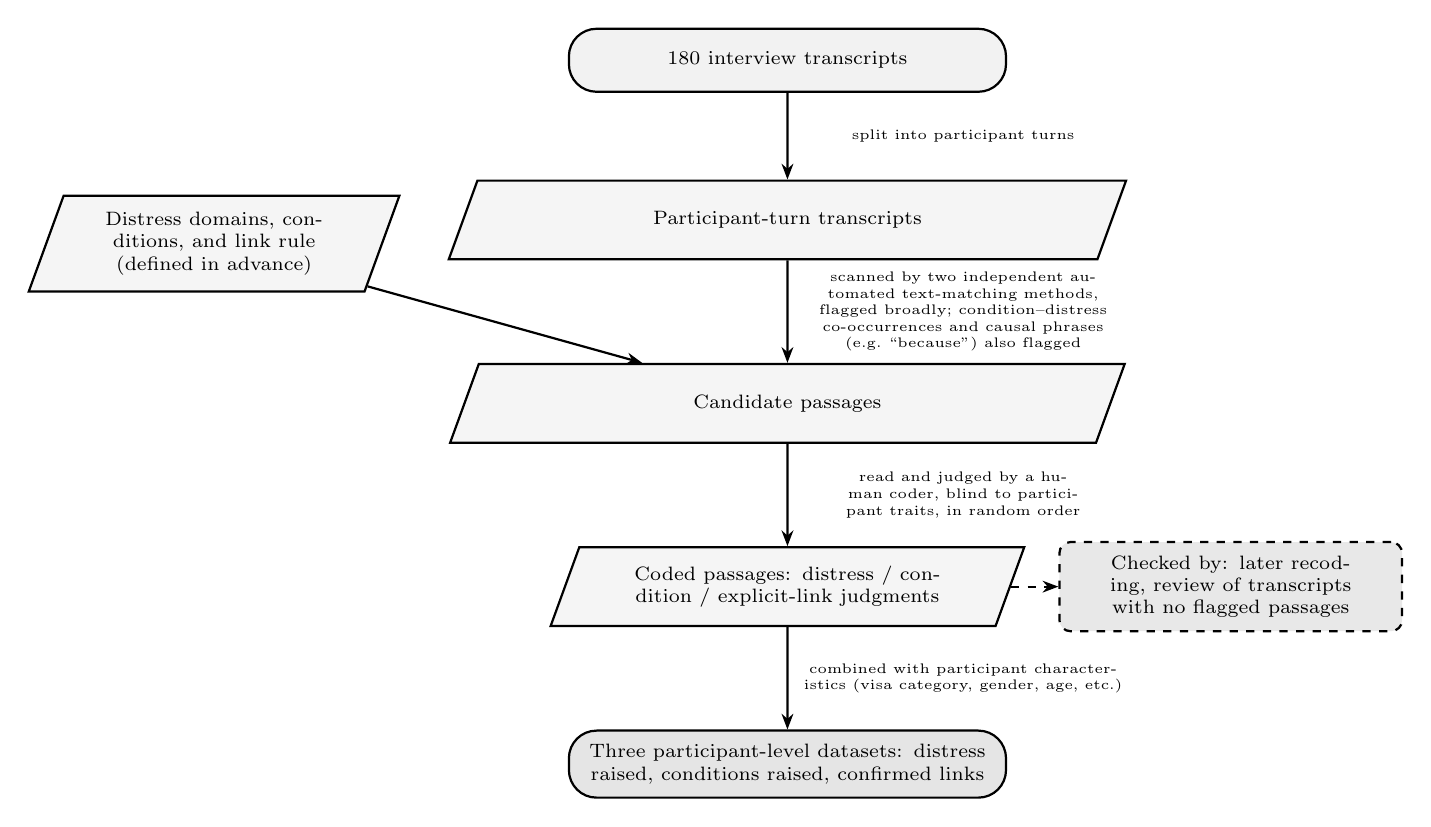
\begin{tikzpicture}[
    node distance=0.5cm and 1.1cm,
    terminal/.style={
        rectangle,
        rounded corners=10pt,
        draw=black,
        thick,
        text width=5.2cm,
        minimum height=0.8cm,
        align=center,
        font=\scriptsize,
        fill=gray!10,
        inner sep=5pt
    },
    data/.style={
        trapezium,
        trapezium left angle=70,
        trapezium right angle=110,
        draw=black,
        thick,
        text width=4.6cm,
        minimum height=1cm,
        align=center,
        font=\scriptsize,
        fill=gray!8,
        inner sep=6pt
    },
    dataS/.style={
        trapezium,
        trapezium left angle=70,
        trapezium right angle=110,
        draw=black,
        thick,
        text width=3.4cm,
        minimum height=1cm,
        align=center,
        font=\scriptsize,
        fill=gray!8,
        inner sep=6pt
    },
    note/.style={
        rectangle,
        rounded corners,
        draw=black,
        thick,
        dashed,
        text width=4.0cm,
        minimum height=1.1cm,
        align=center,
        font=\scriptsize,
        fill=gray!18,
        inner sep=5pt
    },
    arr/.style={-{Stealth[length=2mm]}, thick},
    darr/.style={-{Stealth[length=2mm]}, thick, dashed},
    lbl/.style={font=\tiny, align=center, text width=4.2cm},
]

% nodes
\node[terminal] (transcript) {180 interview transcripts};

\node[data, below=1.1cm of transcript] (turns)
    {Participant-turn transcripts};

\node[dataS, left=1.0cm of turns, yshift=-0.3cm] (spec)
    {Distress domains, conditions, and link rule (defined in advance)};

\node[data, below=1.3cm of turns] (candidates)
    {Candidate passages};

\node[data, below=1.3cm of candidates] (coded)
    {Coded passages: distress / condition / explicit-link judgments};

\node[note, right=0.6cm of coded] (checks)
    {Checked by: later recoding,
    review of transcripts with no flagged passages};

\node[terminal, below=1.3cm of coded, fill=gray!20] (final)
    {Three participant-level datasets: distress raised,
    conditions raised, confirmed links};

% arrows
\draw[arr] (transcript) --
    node[lbl, right] {split into participant turns}
    (turns);

\draw[arr] (turns) --
    node[lbl, right] {
        scanned by two independent automated text-matching methods,
        flagged broadly; condition--distress co-occurrences and
        causal phrases (e.g.\ ``because'') also flagged
    }
    (candidates);

\draw[arr] (spec) -- (candidates);

\draw[arr] (candidates) --
    node[lbl, right] {
        read and judged by a human coder,
        blind to participant traits, in random order
    }
    (coded);

\draw[darr] (coded) -- (checks);

\draw[arr] (coded) --
    node[lbl, right] {
        combined with participant characteristics
        (visa category, gender, age, etc.)
    }
    (final);

\end{tikzpicture}%
}

\caption{Coding Flow Chart.}
\label{fig:flow_chart}

\end{figure}

The coded passages are combined into three datasets at the participant level: one recording which distress domains each
participant raised, one recording which conditions each participant raised, and one recording every confirmed link
between a condition and a distress domain, noting whether the condition was something the interview guide specifically
asked about or something the participant brought up unprompted. These are merged with participant characteristics
collected separately, including visa category, gender, age, time in the United States, national origin, parental
status, and household position.

The main analysis compares how often participants in each visa category, gender, and household position raise each
distress domain, since this comparison requires no modeling assumptions and speaks most directly to the first research
question. Before comparing groups, we check whether participants who talked longer in their interviews simply raised
more topics of every kind, since this could create an apparent difference between groups if interview length itself
differs by visa category or gender; where it does, interview length is accounted for in the comparison. As a secondary
analysis, we test statistically whether participants fall into distinct groups defined by which combination of distress
domains they raise, rather than simply differing in how much distress they express overall; where the data instead show
only a difference in overall level, we report a simple count of domains raised per participant instead. Finally, the
confirmed links between conditions and distress are summarized in a simple chart showing how often each condition is
linked to each type of distress, shown separately by visa category and separately for links the interview guide asked
about versus links participants raised unprompted, and illustrated with quotations organized by condition.

\section{Implications}
[TBA: significance; policy implication]

\vspace{2em}
\noindent\rule{\linewidth}{0.4pt}

\vspace{0.5em}
\noindent\emph{Extended abstract word count: [x]. Tables: 1. Figures: 1.}

\printbibliography
\end{document}